\clearpage
\section{Signal models and efficiencies\label{sec:signal}}

fill 

\subsection{Introduction}

As mentioned in section~\ref{theory}, SUSY is a theory of many particles
and parameters.  Simplifed models (SMS) have been derived~\cite{Alwall:2008ag,Alwall:2008va,sms}
which reduce both particles and parameters at the cost of losing 
generality of the full SUSY model. Yet, SMS models are benificial experimentally,
as they provide clear signatures to search for.  Two SMS models have been studied
1. T2cc: pair produced stop sparticles each decaying into a charm quark and a neutralino.
2. T2tt: pair produced stop sparticles each decaying into a top quart and a neutralino.

Event samples for the simplified models are generated by the CMS SUSY MC group
[REF] at leading order with \MADGRAPH~\cite{madgraph}. I%nclusive, process-dependent,
%next-to-leading order calculations with next-to-leading logarithmic
%corrections~\cite{susy-nlo-nll} (NLO+NLL) of SUSY production cross
%sections are obtained with the program \PROSPINO~\cite{Beenakker1996ch} and
%\verb!CTEQ6L!~\cite{Pumplin:2002vw} parton distribution functions. 
%The \texttt{FastSim} framework is used, and the simulated signal events
%include multiple interactions per LHC bunch crossing (pileup) with the
%distribution of reconstructed vertices that match the one observed in
%data.
The MC samples are listed in Section~\ref{sec:samples}.

The SMS samples are produced in bins of stop mass (mStop) and neutralino
mass (mLSP). The analysis efficieny is studied in the usual \njet, \nb binning
but due to computational limitations not all categories are used to set 
a limit on a given model. The choice of categories for a model is made by
computing the expected upper limit on the signal cross-section for each
category seperatly using the much quicker asymptotic method [REF]. The categories
are ranked by their expected upper limit. Depending on the number of 
mass bins and number of events per bin, two or more categories with the 
higest rank are chosen.

The simplified models, along with the event categories considered for each,
is summarised in Table~\ref{tab:simplified-models}.


\begin{table}[h!]
  \caption{A summary of the simplified models considered for
    interpretation. The event categories considered for each model are
    listed.}  
  \label{tab:simplified-models}
  \setlength{\extrarowheight}{2.5pt}
  \centering
  \begin{tabular}{ llcc }
    \hline
    \hline
    Model             & Production/decay mode & (\njet,\nb) event categories considered        \\ 
    \hline
    \texttt{T2cc}     & \Ttwocc               & (2--3,0), ($\geq 4$,0), ($\geq 4$,1) \\ % (2--3,1), 
    \texttt{T2tt}     & \Ttwott               & ($\leq 3$,1), ($\leq 4$,2) \\
    \hline
    \hline
  \end{tabular}
\end{table}

\subsection{Efficiency times acceptance\label{sec:t2cc-eff}}

The signal efficiency times acceptance is measured in the same binning
as the analysis binning (\njet,\nb,\scalht). To reduce the number of
figures in this section to a manageable level, the total efficiency for
only the relevant event categories and inclusive selection on 
\scalht ($>200\gev$) is shown. 
  
Figure~\ref{fig:sms-eff-t2cc} (Appendix~\ref{app:t2cc}) shows the
expected signal efficiency times acceptance for the hadronic selection
\texttt{T2cc} in the four most sensitive (\njet,\nb) event categories:
(2--3,0), (2--3,1), ($\geq 4$,0), and ($\geq 4$,1). 

\begin{figure}[h!]
  \begin{center}
    \subfigure[Hadronic Selection Efficiency, (2--3,0)]{
      \includegraphics[width=0.4\textwidth,page=6]{figures/sms/t2cc/v1/T2cc_eff}
    } 
    \subfigure[Hadronic Selection Efficiency, (2--3,1)]{
      \includegraphics[width=0.4\textwidth,page=7]{figures/sms/t2cc/v1/T2cc_eff}
    } 
    \subfigure[Hadronic Selection Efficiency, ($\geq 4$,0)]{
      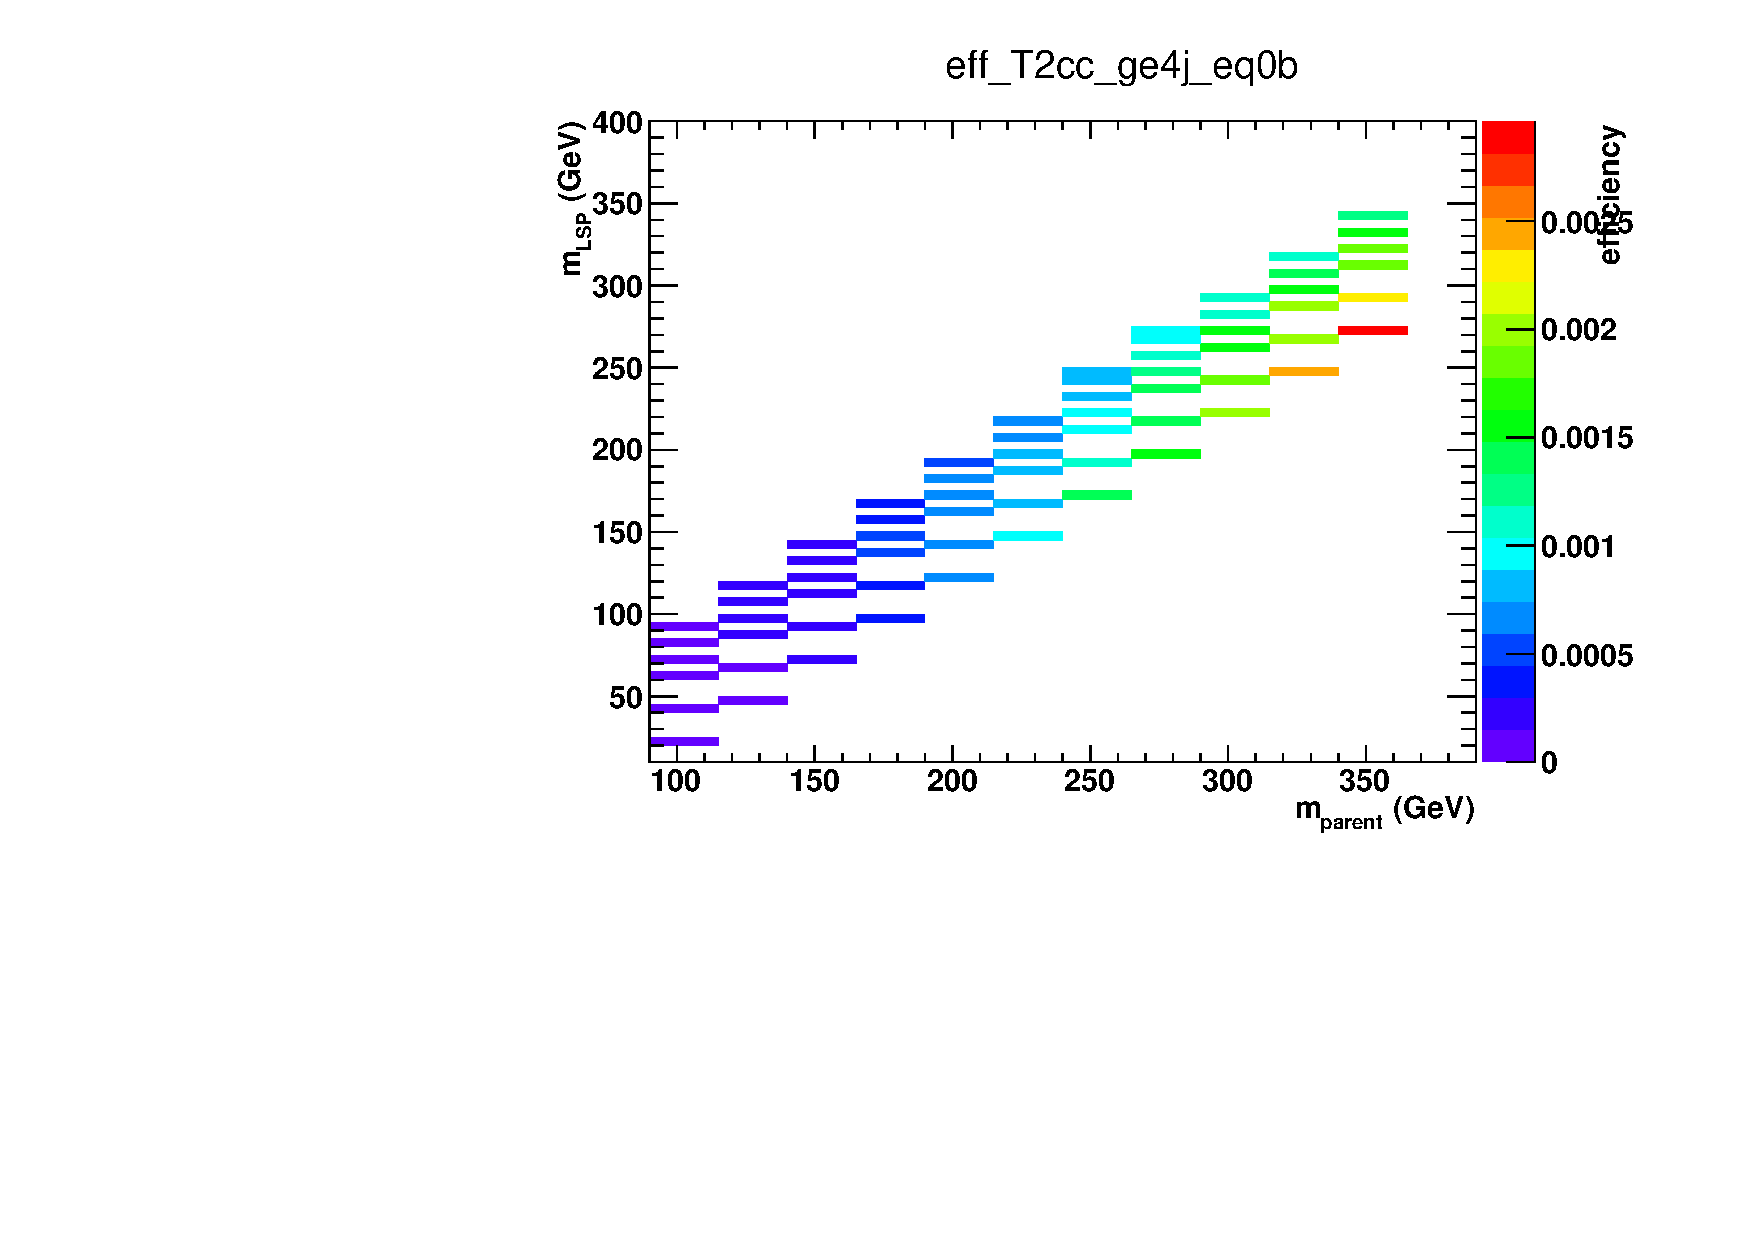
\includegraphics[width=0.4\textwidth,page=1]{figures/sms/t2cc/v1/T2cc_eff}
    } 
    \subfigure[Hadronic Selection Efficiency, ($\geq 4$,1)]{
      \includegraphics[width=0.4\textwidth,page=2]{figures/sms/t2cc/v1/T2cc_eff}
    } 
    \caption{Hadronic selection efficiency times acceptance for \texttt{T2cc}
      for the relevant event categories defined by \njet and \nb.
      Note the different z-axis scales.}
    \label{fig:sms-eff-t2cc}
  \end{center}
\end{figure}

\begin{figure}[h!]
  \begin{center}
    \subfigure[\njetlow, $\nb = 1$.]{
     \includegraphics[width=0.48\textwidth,page=2]{figures/sms/t2tt/v1/t2tt_pfJet_totalUnc.pdf}
    }
    \subfigure[\njetlow, $\nb = 2$.]{
     \includegraphics[width=0.48\textwidth,page=3]{figures/sms/t2tt/v1/t2tt_pfJet_totalUnc.pdf}
    }\\       
    \caption{\label{fig:sms-total-t2tt}The total systematic
      uncertainty in the signal efficiency times acceptance for all
      relevant event categories for the \texttt{T2tt} intepretation.}
  \end{center}
\end{figure}

%The choice of which categories to use is made by inspecting
%Figure~\ref{fig:sms-t2cc-sig} (Appendix~\ref{app:t2cc}), which shows
%the expected significance per signal region bin following the
%injection of signal at the theoretical QCD production cross section
%for the \verb!T2cc! model mass points $m_{\sTop} = 250\gev$ and
%$m_{\rm LSP} = 170\gev$ (Top) and $m_{\rm LSP} = 240\gev$ (Bottom).
%%$m_{\rm LSP} = 230\gev$ (Middle)

The efficiencies are typically at the percent level or less due to
reliance on hard-\Pt jets from initial state radiation for acceptance
in the presence of a compressed mass spectrum and soft decay
products. The largest efficiencies for the smallest mass splittings,
$\Delta M = \sim10\gev$, are obtained with the (2--3,0) category,
while for larger mass splittings the (2--3,1), ($\geq 4$,0), and
($\geq 4$,1) categories contribute due to the reduced backgrounds in
these categories. The signal efficiency in the \mj control sample is
negligible with respect to the signal region. By extension, the
relative contamination for the \mmj sample is also considered to be
negligible. Regardless, any potential contamination is accounted for
in the likelihood model.

%\subsection{Efficiency times acceptance for T2\_4body\label{sec:t2_4body-eff}}
%
%Figure~\ref{fig:sms-eff-t2_4body} (Appendix~\ref{app:t2_4body}) shows
%the expected signal efficiency times acceptance for the signal region
%and \mj control sample (\ie, signal contamination) for the model
%\verb!T2_4body! for the relevant event categories defined in terms of
%\njet and \nb. Several (\njet,\nb) categories are considered. As for
%\verb!T2cc!, the (2--3,0) category provides the largest efficiencies,
%typically at the percent level, for the smallest mass splittings. The
%(2--3,1), ($\geq 4$,0), and ($\geq 4$,1) categories contribute for
%larger mass splittings, but the efficencies are very low, typically at
%or below the per mille level, due to the presence of leptons in the
%final state. As a result, the signal contamination in the \mj and \mmj
%control samples, with respect to the signal region, can be
%non-negligible for models with larger mass splittings, but the S/B is
%still relatively small due to the increased background acceptance of
%the muon control samples (in the absence of an \alphat
%requirement). Further, any potential signal contamination is fully
%accounted for in the likelihood model.

\clearpage
\section{Systematic uncertainties on signal efficiency times 
  acceptance\label{sec:sms-syst}}

\subsection{Introduction} 

The systematic uncertainty in the signal acceptance times efficiency
is determined per mass point per event category (\njet,\nb), but inclusively
in \scalht to gain statistical power. This section details the methods 
used to determine the magnitude of the systematic uncertainties to be applied. 
Four sources of uncertainty are measured: the jet energy scale,
the parton distribution functions, initial state radiation and b-tag scale
factors. Two other uncertainties are quoted: the uncertainty in the luminosity, 
measurment and the ``dead ECAL'' filter used in the candidate signal
event selection. Each contribution is considered to be independent 
and all contributions are summed in quadrature to obtain a total 
systematic uncertainty per mass point per category.

The following sub-sections provide an overview of the various sources of
uncertainty, before details on specific models are provided. 
%
%\subsection{Shape systematics} 
%
%As stated above, the effect of various sources of uncertainty on the
%experimental acceptance times efficiency is determined per model per
%event category. However, some simplifications have been made in order
%to rationalise the process to determine the systematic uncertainties. 
%
%The systematic uncertainties presented below are determined per model
%per event category for an inclusive selection $\scalht >
%200\gev$. They reflect the effect on signal acceptance due to changes
%in the various sources of uncertainties. The resulting systematic is
%taken as a flat contribution across all \scalht bins for a given
%category. Clearly, this an overestimate for the higher \scalht bins,
%for which the probability to lose events (\ie fall below $\scalht >
%200\gev$) is significantly reduced. Further, events can migrate
%between (\njet,\nb) categories and not be lost, but again this
%approach does not account for category migration and overestimates the
%effect. Studies have been perform to check that the above approach is
%indeed appropriate, such as the effect of the dominant uncertainties
%(\eg JES, ISR, and PDF) on the \scalht shape for a model near to the
%expected limit contour. These studies are summarised below, which
%support the assumption that that systematic uncertainties in the
%signal acceptance times efficiency, if taken as a flat contribution
%across all \scalht bins, covers the uncertainty in the \scalht shape.
%
\subsection{PDF uncertainties\label{sec:pdf-sets}}

The simulated signal events were produced with the \verb!CTEQ6L1! PDF
set by default.  As recommended by PDF4LHC~\cite{pdf4lhc}, the uncertainty
in signal efficiency due to knowledge of the PDFs is obtained by comparing 
the signal efficiency with that obtained with three newer alternative PDF 
sets: \verb!CT10!, \verb!NNPDF2.1!, and \verb!MSTW2008!. Using the envelope
formula in the reference, a single value is calculated from the three alternate
PDF sets. Figures ~\ref{fig:sms-pdf-t2cc} and ~\ref{fig:sms-pdf-t2tt} in Appendix
 ~\ref{app:signal} summarize the uncertainty measured for T2cc and T2tt 
for the relevant categories. 

\subsection{Jet energy scale\label{sec:sms-syst-jes}}

The relative change in the signal efficiency times acceptance is
determined when varying the energy of all jets in an event up or down
according to a \pt- and $\eta$-dependent jet energy scale uncertainty
(\ie vary the event scale up and down), as recommended by the JetMET
POG. This procedure is followed per mass point per event category for
an inclusive selection on \scalht ($> 375\gev$). 

\subsection{Initial state radiation\label{sec:sms-syst-isr}}

Signal samples produced with \MADGRAPH exhibit discripencies that 
have been attributed to the mismodelling of initial state radiation.
These discripencies are corrected as recommended by the SUSY 
PAG~\cite{susy-isrrw}. As per prescripton, events are reweighted
according to the vectorial sum of the momenta of the pair-produced
sparticles. The sparticle-system \Pt dependent weights are summarized in  
Table~\ref{tab:sms-syst-isr-factors}.   In addition to the central weight, 
further variations about the central weight according to the uncertainty 
in the weight is applied in order to determine the systematic uncertainty
associated with the correction. These systematic uncertainties are determined per
mass point per event category for an inclusive selection on \scalht
($> 375\gev$).
The resulting systematic uncertainties are largest near the diagonal
where selected events contain significant amounts of boost due to the
presence of initial state radiation. 

\begin{table}[!h]
  \caption{Sparticle system \Pt dependent corrections and systematic
    weight variations.} 
  \label{tab:sms-syst-isr-factors}
  \centering
  \footnotesize
  \begin{tabular}{ lcc }
    \hline
    Sparticle system \Pt (GeV) & Central Weight & Systematic Variation \\
    \hline
    $0 < \Pt < 120$            & 1.00           & $\pm$ 0.0            \\
    $120 < \Pt < 150$          & 0.95           & $\pm$ 0.05           \\
    $150 < \Pt < 250$          & 0.90           & $\pm$ 0.10           \\
    $\Pt > 250$                & 0.80           & $\pm$ 0.20           \\
    \hline
    \hline
  \end{tabular}
\end{table}

\subsection{b-tag scale factor corrections\label{sec:sms-syst-btag}}

The uncertainty on the btag scale factors described in section [REF]
is calculated by varying the scale factors up and down by their
uncertainty as described in Ref.~\cite{btagpogtwiki}.
where the relevant dependences are implied. Once all events have been
reweighted this way, the yields in each $b$-tag bin represent the
corrected MC yields. 

\subsection{Systematic uncertainties for T2cc\label{sec:sms-t2cc}}

Figure~\ref{fig:sms-pdf-t2cc} (Appendix~\ref{app:t2cc}) shows the
ratio of the signal efficiency times acceptance for the central value
and $\pm1\sigma$ variations of the envelope calculation relative to
the nominal PDF (\verb!CTEQ6L1!)  set used to produce the
\texttt{T2cc} sample. The relative difference (based on the central
value of the envelope calculation) is currently taken as a (symmetric)
systematic uncertainty, which varies in absolute terms within the
range 0--10\% across the \verb!T2cc! mass plane, with the largest
positive changes at the smallest top squark mass of 100\gev. The
systematic uncertainty is determined independently of \njet and \nb
and is used for all \scalht bins (a conservative approach). 

Figure~\ref{fig:sms-jes-t2cc} (Left and Middle) shows the relative
change in the signal efficiency times acceptance for the relevant
categories for the \verb!T2cc! interpretation when varying the energy
of all jets in an event up or down according to a \pt- and
$\eta$-dependent jet energy scale uncertainty (\ie vary the event
scale up and down), as recommended by the JetMET POG. Larger
variations are observed for the higher jet multiplicity category, as
as the jets are softer for the same requirement on \scalht. Also, the
variations may increase with increasing mass splitting as additional
(soft) jets from the decay become hard enough to move within
acceptance. Figure~\ref{fig:sms-jes-t2cc} (Right) also shows the
maximum value from the up and down variations, point-by-point, which
are used as the contribution to the total systematic uncertainty on
the signal efficiency times acceptance. The variations are on average
$\sim5\%$ and $\sim15\%$ for the low and high jet multiplicity bins,
respectively, and largely independent of parent and daughter sparticle
mass. 

Figure~\ref{fig:sms-isr-t2cc} (Left and Middle) shows the relative
change in the signal efficiency times acceptance for the relevant
categories for the \verb!T2cc! interpretation when varying up and down
the sparticle system \Pt-dependent corrections by their
uncertainties. The largest variations, up to $\sim$25\% are observed
for the smallest mass splittings, when the reliance on ISR jets for
acceptance is largest. Figure~\ref{fig:sms-isr-t2cc} (Right) also
shows the maximum value from the up and down variations,
point-by-point, which are used as the contribution to the total
systematic uncertainty on the signal efficiency times acceptance. This
is the most dominant contribution to the total.

Figure~\ref{fig:sms-btag-t2cc} (Left and Middle) shows the relative
change in the signal efficiency times acceptance for the relevant
categories for the \verb!T2cc! interpretation when varying up and down
the scale-factor corrections by their uncertainties. The variations
are anti-correlated for the two \nb categories used by this
interpretation and are generally small, at the level of 1--5\%, with
respect to other contributions.  Figure~\ref{fig:sms-btag-t2cc}
(Right) shows the maximum value from the up and down variations,
point-by-point, which are used as the contribution to the total
systematic uncertainty on the signal efficiency times acceptance.

Table~\ref{tab:sms-syst-t2cc} presents a {\it representative} range of
values for the contribution to the total systematic uncertainty in the
signal efficiency times acceptance for each relevant event
category. An uncertainty of 2.3\% in the integrated luminosity is also
considered. An uncertainty of 4\% from increasing the number of
associated partons (from 2 to 3) in the scan is also considered. The
contribution from PDF uncertainties are determined for an inclusive
selection on \njet and \nb only. Figure~\ref{fig:sms-total-t2cc} shows
the total systematic uncertainty in the \verb!T2cc! mass plane for the
relevant categories.

\begin{table}[h!]
  \caption{Representative ranges for each contribution to the total
    systematic uncertainty in the signal efficiency times acceptance
    for each relevant event category for the \texttt{T2cc}
    interpretation. See text for further details on other
    (fixed) contributions to the total systematic uncertainty. 
    \label{tab:sms-syst-t2cc}
  }   
  \centering
  \begin{tabular}{ lcccccccc }
    \hline
    \hline
    Category   & \multicolumn{2}{c}{(2--3,0)} & \multicolumn{2}{c}{($\geq 4$,0)} & \multicolumn{2}{c}{($\geq 4$,1)} & \multicolumn{2}{c}{($\geq 2$,$\geq 0$)} \\
    Range      & Min.                         & Max.                             & Min.                             & Max. & Min. & Max. & Min. & Max.        \\
    \hline
    PDF        &                              &                                  &                                  &      &      &      & 0.04 & 0.14        \\
    JES        & 0.00                         & 0.08                             & 0.06                             & 0.22 & 0.01 & 0.30 &      &             \\
    ISR        & 0.09                         & 0.21                             & 0.16                             & 0.24 & 0.15 & 0.24 &      &             \\
    b-tag SF   & 0.01                         & 0.02                             & 0.01                             & 0.02 & 0.03 & 0.04 &      &             \\
    Dead ECAL  & 0.02                         & 0.02                             & 0.02                             & 0.02 & 0.02 & 0.02 &      &             \\
    \hline
    Total syst & 0.12                         & 0.21                             & 0.22                             & 0.32 & 0.23 & 0.39 &      &             \\
    \hline
    \hline
  \end{tabular}
\end{table}

\subsection{Systematic uncertainties for T2tt\label{sec:sms-t2tt}}

Figure~\ref{fig:sms-pdf-t2tt} (Appendix~\ref{app:t2tt}) shows the
ratio of the signal efficiency times acceptance for the central value
and $\pm1\sigma$ variations of the envelope calculation relative to
the nominal PDF (\verb!CTEQ6L1!)  set used to produce the
\texttt{T2cc} sample. The relative difference (based on the central
value of the envelope calculation) is currently taken as a (symmetric)
systematic uncertainty, which varies in absolute terms within the
range 0--10\% across the \verb!T2cc! mass plane, with the largest
positive changes at the smallest top squark mass of 100\gev. The
systematic uncertainty is determined independently of \njet and \nb
and is used for all \scalht bins (a conservative approach). Any
systematic uncertainties resulting from changes in the signal shape
are considered to be negligible, as discussed in
Section~\ref{sec:pdf-sets}

Figures~\ref{fig:sms-jes-up-t2cc} and~\ref{fig:sms-jes-down-t2cc} show
the relative change in the signal efficiency times acceptance for the
relevant categories for the \verb!T2cc! interpretation when varying
the energy of all jets in an event up or down according to a \pt- and
$\eta$-dependent jet energy scale uncertainty (\ie vary the event
scale up and down), as recommended by the JetMET POG. Larger
variations are observed for the higher jet multiplicity category, as
as the jets are softer for the same requirement on \scalht. Also, the
variations may increase with increasing mass splitting as additional
(soft) jets from the decay become hard enough to move within
acceptance. Figure~\ref{fig:sms-jes-t2cc} shows the maximum value from
the up and down variations, point-by-point, which are used as the
contribution to the total systematic uncertainty on the signal
efficiency times acceptance.

Figures~\ref{fig:sms-isr-up-t2cc} and~\ref{fig:sms-isr-down-t2cc} show
the relative change in the signal efficiency times acceptance for the
relevant categories for the \verb!T2cc! interpretation when varying
(up and down) the sparticle system \Pt-dependent corrections by their
uncertainties. The largest variations, up to $\sim$20\% are observed
for the smallest mass splittings, when the reliance on ISR jets for
acceptance is largest. Figure~\ref{fig:sms-isr-t2cc} shows the maximum
value from the up and down variations, point-by-point, which are used
as the contribution to the total systematic uncertainty on the signal
efficiency times acceptance. This is the most dominant contribution to
the total. 

Figures~\ref{fig:sms-btag-up-t2cc} and~\ref{fig:sms-btag-down-t2cc}
show the relative change in the signal efficiency times acceptance for
the relevant categories for the \verb!T2cc! interpretation when
varying (up and down) the scale-factor corrections by their
uncertainties. The variations are anti-correlated for the two \nb
categories used by this interpretation and are generally small, at the
level of 2--4\%, with respect to other contributions.
Figure~\ref{fig:sms-btag-t2cc} shows the maximum value from the up and
down variations, point-by-point, which are used as the contribution to
the total systematic uncertainty on the signal efficiency times
acceptance. 

The contribution from uncertainties in the efficiency of the
$\mht/\met < 1.25$ requirement is expected to be sub-dominant with
respect to other contributions, and is estimated to be at the level of
0--2\% as discussed in Section~\ref{sec:sms-syst-mht-met}. It is
however useful to inspect the expected efficiency of this requirement
for the \verb!T2cc! model to see if the behaviour is comparable to
that observed in data and the \verb!FullSim!
simulation. Figure~\ref{fig:sms-mht-met-ineff-t2cc} shows the
efficiency of the $\mht/\met < 1.25$ requirement for the relevant
categories for the \verb!T2cc! interpretation. The efficiency is
observed to be $\sim$90--97\% for the region $m_{\rm stop} > 200\gev$
and the smallest mass splittings, dropping to $\sim$80\% for smaller
mass values in the region $100 < m_{\rm stop} < 200\gev$. Lower
efficiencies are observed for the larger mass splittings (and smaller
$m_{\rm stop}$), typically in the range 70--90\%. This is likely due
to soft jets from the SUSY decay within acceptance degrading the
resolution of the \mht variable, hence the requirement on \mht/\met
becomes effectively tighter.

The contribution from uncertainties in the efficiency of the dead ECAL
filter is expected to be sub-dominant with respect to other
contributions, and is estimated to be at the level of 0--2\% as
discussed in Section~\ref{sec:sms-syst-dead-ecal}.
Figure~\ref{fig:sms-dead-ecal-ineff-t2cc} shows the efficiency of the
dead ECAL filter for the relevant categories for the \verb!T2cc!
interpretation. The efficiency is observed to be insensitive to the
mass splitting and increasing from 92\% to 97\% (70\% to 93\%) with
$m_{\rm stop}$ for events satisfying \njetlow (\njethigh).

%The efficiency of the dead ECAL filter is found to be in the range
%80--95\% for the simplified models under consideration. The lower
%efficiencies are typical of models with higher jet-multiplicity
%final-states, such as those arising from gluino-gluino
%pair-production, due to the higher probability of an event having at
%least one mis-measured jet pointing to a region of dead ECAL cells or
%the transition between the ECAL barrel and end-cap regions. The lower
%efficiencies are also typical of models with compressed spectra.

Finally, the \verb!T2cc! sample are produced using \MADGRAPH as the
matrix level generator. The scan is produced with up to two associated
partons at the generator level. Given the relatively high sensitivity
to initial state radiation in the signal phase space, a validation
scan was produced with up to three associated partons. The scan
comprises two mass points with $m_{\rm stop} = 200\gev$ and an LSP
mass of 120\gev and 190\gev in order to cover the full range in mass
splittings (\ie $\Delta m = 10 {\rm and} 80\gev$). The ratio of
acceptances between the 3-parton scan relative to the default 2-parton
scan for these two mass points are shown in
Table~\ref{tab:sms-t2cc-2v3part}. These values are interpreted as
contributions to the systematic uncertainty on the efficiency times
acceptance, and the largest relative change, 4\%, is applied across
the full mass plane for all event categories. 

\begin{table}[!h]
  \caption{Relative change in efficiency times acceptance for the
    2-parton and 3-parton scans. The points have a stop mass of
    200GeV and cover two different deltaM points.}
  \label{tab:sms-t2cc-2v3part}
  \centering
  \begin{tabular}{ lcc }
    \hline
    \hline
    Category     & \multicolumn{2}{c}{$\Delta m$ (GeV)} \\
    \cline{2-3}
                 & 10   & 80                            \\
    \hline
    (2--3,0)     & 0.00 & 0.04                          \\
    (2--3,1)     & 0.02 & 0.04                          \\
    ($\geq 4$,0) & 0.04 & 0.04                          \\
    ($\geq 4$,1) & 0.00 & 0.00                          \\
    \hline
    \hline
  \end{tabular}
\end{table}

Table~\ref{tab:sms-syst-t2cc} presents a {\it representative} range of
values for the contribution to the total systematic uncertainty in the
signal efficiency times acceptance for each relevant event
category. An uncertainty of 2.3\% in the integrated luminosity is also
considered. An uncertainty of 4\% from increasing the number of
associated partons (from 2 to 3) in the scan is also considered. The
contribution from PDF uncertainties are determined for an inclusive
selection on \njet and \nb only. Figure~\ref{fig:sms-total-t2cc} shows
the total systematic uncertainty in the \verb!T2cc! mass plane for the
relevant categories.

\begin{table}[h!]
  \caption{Representative ranges for each contribution to the total
    systematic uncertainty in the signal efficiency times acceptance
    for each relevant event category for the \texttt{T2cc}
    interpretation. See text for further details on other
    (fixed) contributions to the total systematic uncertainty. 
    \label{tab:sms-syst-t2cc}
  }   
  \centering
  \begin{tabular}{ lcccccccc }
    \hline
    \hline
    Category   & \multicolumn{2}{c}{(2--3,0)} & \multicolumn{2}{c}{($\geq 4$,0)} & \multicolumn{2}{c}{($\geq 4$,1)} & \multicolumn{2}{c}{($\geq 2$,$\geq 0$)} \\
    Range      & Min.                         & Max.                             & Min.                             & Max. & Min. & Max. & Min. & Max.        \\
    \hline
    PDF        &                              &                                  &                                  &      &      &      & 0.04 & 0.14        \\
    JES        & 0.00                         & 0.08                             & 0.06                             & 0.22 & 0.01 & 0.30 &      &             \\
    ISR        & 0.09                         & 0.21                             & 0.16                             & 0.24 & 0.15 & 0.24 &      &             \\
    b-tag SF   & 0.01                         & 0.02                             & 0.01                             & 0.02 & 0.03 & 0.04 &      &             \\
    \mht/\met  & 0.02                         & 0.02                             & 0.02                             & 0.02 & 0.02 & 0.02 &      &             \\
    Dead ECAL  & 0.02                         & 0.02                             & 0.02                             & 0.02 & 0.02 & 0.02 &      &             \\
    \hline
    Total syst & 0.12                         & 0.21                             & 0.22                             & 0.32 & 0.23 & 0.39 &      &             \\
    \hline
    \hline
  \end{tabular}
\end{table}

